\documentclass[aspectratio=169,unicode,dvipdfmx,14pt]{beamer}


\usepackage{url}
\usepackage{bm}
\usepackage{amsmath}
\usepackage{amssymb}
\usepackage{mathtools}
\usepackage{graphicx}
\usepackage[absolute,overlay]{textpos}
\usepackage{hyperref}
\usepackage{listings}
\usepackage{changepage}
\usepackage{lipsum}


\usefonttheme[onlymath]{serif}

\DeclareMathOperator*{\argmax}{argmax}

\DeclarePairedDelimiterX{\infdivx}[2]{(}{)}{%
  #1\;\delimsize\|\;#2%
}
\newcommand{\infdiv}{D_{\scriptsize \mbox{KL}}\infdivx}
\DeclarePairedDelimiter{\norm}{\lVert}{\rVert}

\hypersetup{
	setpagesize=false,
	bookmarksnumbered=true,%
	bookmarksopen=true,%
	colorlinks=true,%
	linkcolor=blue,
	citecolor=red,
}

\newcommand\FontMath{\fontsize{10}{12}\selectfont}
\renewcommand{\baselinestretch}{1.3}
\renewcommand{\familydefault}{\sfdefault}
\renewcommand{\kanjifamilydefault}{\gtdefault}
\usepackage[deluxe, expert]{otf}

\setbeamertemplate{navigation symbols}{}
\setbeamertemplate{footline}[frame number]
\setbeamerfont{footline}{size={\fontsize{15}{15}}}

\setbeamerfont{author}{size=\Large}
\setbeamerfont{institute}{size=\normalsize\itshape}
\setbeamerfont{title}{size=\huge}
\setbeamerfont{subtitle}{size=\LARGE\normalfont\slshape}


\title{ \\隠れマルコフモデル}
\author{\texorpdfstring{正田 備也\newline\href{mailto:masada@rikkyo.ac.jp}{masada@rikkyo.ac.jp}}{正田 備也}}
\date{}

\begin{document}

\begin{frame}
\titlepage
\end{frame}

\section{マルコフモデル}

\begin{frame}\frametitle{Contents}
\Large \tableofcontents[currentsection]
\end{frame}

\begin{frame}{マルコフモデル}
\begin{itemize}
\item $\bm{z} = (z_1,\ldots,z_T)$という確率変数の列がある
\item $z_t$は、状態の集合$\mathcal{S} = \{ s_1, \ldots, s_K \}$の要素を値として取る
\begin{itemize}
\item[例.] 天候の集合$\mathcal{S} = \{ s_{\mbox{\scriptsize sun}}, s_{\mbox{\scriptsize cloud}}, s_{\mbox{\scriptsize rain}} \}$
\end{itemize}
\item 以下の単純マルコフ性の仮定をおく
\vspace{-.1in}
\begin{align}
p(z_i =s | z_1,\ldots, z_{i-1}) = p(z_i =s | z_{i-1}) \mbox{ for all $s \in \mathcal{S}$}
\end{align}
\item $s_k$から$s_l$に遷移する確率$p(z_t=s_l|z_{t-1}=s_k)$は、全ての$t$で等しいと仮定(斉時性の仮定)し、この確率を$A_{s_k,s_l}$と書く
\begin{itemize}
\item $\sum_{l=1}^K A_{s_k, s_l} = 1$が、すべての$k$で成り立つ
\end{itemize}
\item 便宜的に初期状態を確率変数$z_0$で表し、その値を$s_0$とする
\begin{itemize}
\item $A_{s_k,s_0} = 0$が、すべての$k$について成り立つ
\end{itemize}
\end{itemize}
\end{frame}

\begin{frame}{遷移行列}
\begin{itemize}
\item 遷移確率をまとめて、遷移行列$A$として書く
\item[例.] 天候の状態の集合$\mathcal{S} = \{ s_0, s_{\mbox{\scriptsize sun}},
s_{\mbox{\scriptsize cloud}}, s_{\mbox{\scriptsize rain}} \}$
\begin{align}
A = \left[
    \begin{array}{ccccc}
 & s_0 & s_{\mbox{\scriptsize sun}} & s_{\mbox{\scriptsize cloud}} & s_{\mbox{\scriptsize rain}} \\
s_0 & 0 & 0.33 & 0.33 & 0.33 \\
s_{\mbox{\scriptsize sun}} & 0 & 0.8 & 0.1 & 0.1 \\
s_{\mbox{\scriptsize cloud}} & 0 & 0.2 & 0.6 & 0.2 \\
s_{\mbox{\scriptsize rain}} & 0 & 0.1 & 0.2 & 0.7
    \end{array}
  \right]
\end{align}
\vspace{-.1in}
\begin{itemize}
\item[cf.] \href{http://cs229.stanford.edu/section/cs229-hmm.pdf}{http://cs229.stanford.edu/section/cs229-hmm.pdf}
\end{itemize}
\end{itemize}
\end{frame}

\begin{frame}{状態列の尤度}
\begin{itemize}
\item 状態の列$\bm{z}_{1:T}\equiv(z_1,\ldots,z_T)$の尤度$p(\bm{z}_{1:T})$は
\begin{align}
p(\bm{z}_{1:T};A) & = p(z_1,\ldots,z_T;A) \notag \\
& = p(z_0, z_1,\ldots,z_T;A) \notag \\
& = p(z_T | z_{T-1},\ldots,z_1;A) \cdots p(z_2|z_1;A) p(z_1|z_0;A) \notag \\
& = p(z_T | z_{T-1};A) \cdots p(z_2|z_1;A) p(z_1|z_0;A) \notag \\
& = \prod_{t=1}^T p(z_t | z_{t-1};A) = \prod_{t=1}^T A_{z_{t-1}, z_t}
\label{eq:seq_LH}
\end{align}
\vspace{-.1in}
\begin{itemize}
\item[問.] どこで単純マルコフ性の仮定を使っているか?
\end{itemize}
\end{itemize}
\end{frame}

\begin{frame}{マルコフモデルの最尤推定}
\FontMath
$\ln p(\bm{z}_{1:T};A)$を最大化することで$A$を推定する。
\begin{align}
\ln p(\bm{z}_{1:T};A) 
= \sum_{t=1}^T \ln A_{z_{t-1}, z_t}
= \sum_{t=1}^T \sum_{l=1}^K \sum_{k=1}^K \mathbbm{1}(z_{t-1}=s_l \wedge z_t=s_k) \ln A_{s_l,s_k}
\end{align}
$\mathbbm{1}(\cdot)$は、括弧内の命題が真のとき$1$、偽のとき$0$、という意味だとする。
\vspace{-0.05in}
\begin{align}
\mathcal{L}(A,\{ \lambda_k \}) = 
\sum_{t=1}^T \sum_{l=1}^K \sum_{k=1}^K \mathbbm{1}(z_{t-1}=s_l \wedge z_t=s_k) \ln A_{s_l,s_k}
+ \sum_{l=1}^K \lambda_l \bigg( 1 - \sum_{k=1}^K A_{s_l,s_k} \bigg) 
\end{align}
\vspace{-0.1in}
\begin{align}
\frac{\partial \mathcal{L}(A,\{ \lambda_k \})}{\partial A_{s_l,s_k}}
= \frac{ \sum_{t=1}^T \mathbbm{1}(z_{t-1}=s_l \wedge z_t=s_k) }{ A_{s_l,s_k} } - \lambda_l
\end{align}
$\frac{\partial \mathcal{L}(A,\{ \lambda_k \})}{\partial A_{s_l,s_k}} = 0$より
$A_{s_l,s_k} \propto \sum_{t=1}^T \mathbbm{1}(z_{t-1}=s_l \wedge z_t=s_k)$で、
$\sum_{k=1}^K A_{s_l,s_k}=1$だから
\begin{align}
\therefore A_{s_l,s_k} = \frac{ \sum_{t=1}^T \mathbbm{1}(z_{t-1}=s_l \wedge z_t=s_k) }
{ \sum_{k=1}^K \sum_{t=1}^T \mathbbm{1}(z_{t-1}=s_l \wedge z_t=s_k) }
= \frac{ \sum_{t=1}^T \mathbbm{1}(z_{t-1}=s_l \wedge z_t=s_k) }
{ \sum_{t=1}^T \mathbbm{1}(z_{t-1}=s_l) }
\end{align}
\end{frame}

\section{隠れマルコフモデル}

\begin{frame}\frametitle{Contents}
\Large \tableofcontents[currentsection]
\end{frame}

\begin{frame}{例. アイスクリームの売上で温暖化を研究}
\begin{itemize}
\item あなたは西暦2799年の世界に生きており、地球温暖化の研究をしている
\item 歴史的な資料の中から、2020年夏の毎日のアイスクリームの売上の記録が見つかった
\item この記録を元に、2020年夏の毎日の天候を推定したい
\item ただし、アイスクリームの売上は天候だけに依存すると仮定
\begin{itemize}
\item \href{https://web.stanford.edu/~jurafsky/slp3/A.pdf}{https://web.stanford.edu/\~{}jurafsky/slp3/A.pdf}
\end{itemize}
\end{itemize}
\end{frame}


\begin{frame}{隠れマルコフモデルHMM; hidden Markov model}
\begin{itemize}
\item 状態$z_t$は観測できず、各状態が生成する結果$x_t$だけが観測できるとする
\begin{itemize}
\item このとき、状態を表す確率変数$z_t$は潜在変数latent variableとなる
\end{itemize}
\item 隠れ状態の列$\bm{z}_{1:T}=(z_1,\ldots,z_T)$は、上述のとおり、単純マルコフ性と斉時性を持つと仮定する
\item 時点$t$での観測結果を、確率変数$x_t$で表す
\item 観測データ$x_t$について、以下のような独立性の仮定をおく
\begin{align}
p(x_t=v_w| \bm{x}_{1:T},\bm{z}_{1:T}) = p(x_t=v_w|z_t=s_k)
\end{align}
\vspace{-.2in}
\begin{itemize}
\item つまり、時点$t$の観測値は、同じ時点の隠れ状態だけに依存する
\end{itemize}
\end{itemize}
\end{frame}

\begin{frame}{観測データがカテゴリカルデータの場合}
\begin{itemize}
\item ここでは、観測データはカテゴリカルデータだとする
\begin{itemize}
\item 観測データが連続値で、$p(x_t|z_t)$が、例えば正規分布の場合、以下の議論がどうなるか、考えてみよう
\end{itemize}
\item 隠れ状態$s_k$がであるときの、アイテム$v_w$の出現確率$p(x_t=v_w|z_t=s_k)$を、$B_{s_k,v_w}$と書くことにする
\begin{itemize}
\item $(B_{s_k,v_1}, \ldots, B_{s_k,v_W})$は、状態$s_k$に対応するカテゴリカル分布の、パラメータである
\item $\sum_{w=1}^W B_{s_k,v_w} = 1$が成り立つ
\end{itemize}
\item 隠れマルコフモデルにおけるパラメータ推定では、$A$と$B$を推定することになる
\end{itemize}
\end{frame}

\begin{frame}{混合分布モデルと隠れマルコフモデル}
\begin{itemize}
\item 混合分布モデル
\begin{textblock*}{0.4\linewidth}(260pt, 40pt)
    \centering
    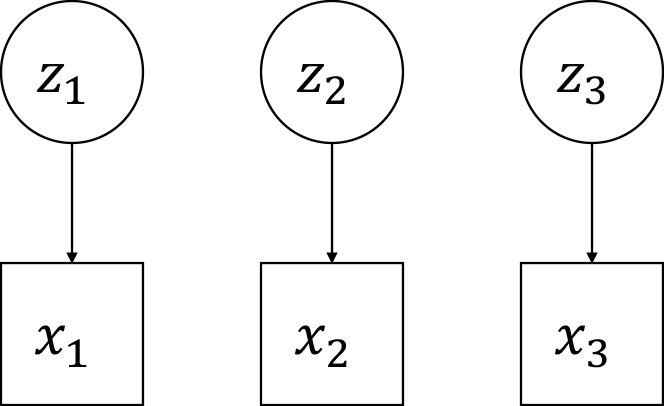
\includegraphics[width=\linewidth]{HMM1.jpg}
\end{textblock*}
\begin{itemize}
\item 隠れ変数$z_i$は独立
\end{itemize}
\vspace{1in}
\item 隠れマルコフモデル
\begin{textblock*}{0.4\linewidth}(225pt, 145pt)
    \centering
    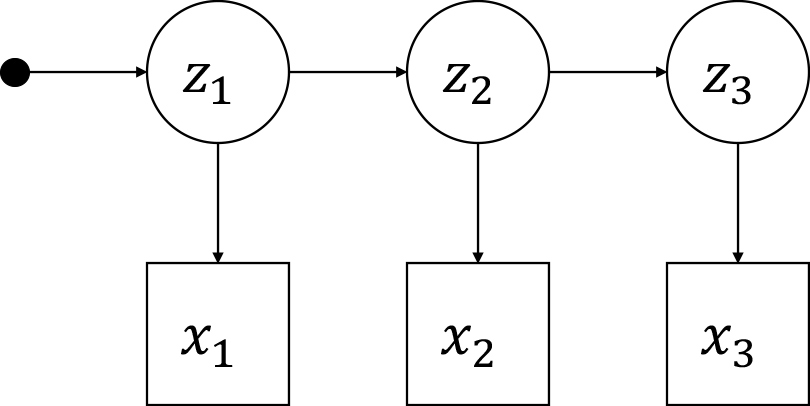
\includegraphics[width=1.25\linewidth]{HMM2.jpg}
\end{textblock*}
\begin{itemize}
\item 隠れ変数$z_t$の間に依存関係
\item 線形で一方向的な依存関係
\end{itemize}
\end{itemize}
\end{frame}

\begin{frame}{同時分布}
\begin{itemize}
\item 隠れマルコフモデルでの観測変数と隠れ変数の同時分布は
\begin{align}
p(\bm{x}_{1:T}, \bm{z}_{1:T};A,B)
& = p(\bm{x}_{1:T} | \bm{z}_{1:T};B) p(\bm{z}_{1:T};A)
\notag \\ &
= \prod_{t=1}^T p(x_t|z_t;B) \times \prod_{t=1}^T p(z_t|z_{t-1};A)
\notag \\ &
= \prod_{t=1}^T B_{z_t,x_t} \times \prod_{t=1}^T A_{z_{t-1},z_t}
\end{align}
\begin{itemize}
\item 状態列の確率$p(\bm{z}_{1:T})$の部分は、式\eqref{eq:seq_LH}と同じ
\item ただし、隠れマルコフモデルでは$z_t$は潜在変数
\end{itemize}
\end{itemize}
\end{frame}


\begin{frame}{観測データの尤度}
\begin{itemize}
\item 観測データの尤度$p(\bm{x}; A,B)$は
\begin{align}
p(\bm{x}; A,B) &
= \sum_{\bm{z}} p(\bm{x},\bm{z}; A,B)
\notag \\
& = \sum_{z_1 \in \mathcal{S}} \cdots \sum_{z_T \in \mathcal{S}}
\bigg( \prod_{t=1}^T p(x_t|z_t;B) \bigg) \bigg( \prod_{t=1}^T p(z_t|z_{t-1};A) \bigg)
\notag \\ & 
= \sum_{z_1 \in \mathcal{S}} \cdots \sum_{z_T \in \mathcal{S}} \bigg( \prod_{t=1}^T B_{z_t,x_t} \bigg)
\bigg( \prod_{t=1}^T A_{z_{t-1},z_t} \bigg)
\end{align}
\vspace{-.1in}
\begin{itemize}
\item だが、この式をそのまま使って計算すると、計算量が$O(|\mathcal{S}|^T) = O(K^T)$であるため、
非現実的な計算時間になる
\end{itemize}
\end{itemize}
\end{frame}

\section{隠れマルコフモデルの尤度計算}

\begin{frame}\frametitle{Contents}
\Large \tableofcontents[currentsection]
\end{frame}


\begin{frame}{Forward procedure}
\begin{itemize}
\item HMMのデータ尤度$p(\bm{x}; A,B)$は、動的計画法の一種である
forward procedureによって、効率的に計算できる
\begin{itemize}
\item[cf.] \href{https://web.stanford.edu/~jurafsky/slp3/A.pdf}{https://web.stanford.edu/\~{}jurafsky/slp3/A.pdf}
\end{itemize}
\item 時点$t$までのデータ列$(x_1,\ldots,x_t)$の確率と、
時点$t$での隠れ状態$z_t$が$s_k$である確率の同時確率を、$\alpha_t(k)$とおく。つまり
\begin{align}
\alpha_t(k) \equiv p(x_1,\ldots, x_t, z_t=s_k; A, B)
\end{align}
\item すると、データ尤度を以下のように表すことができる
\begin{align}
p(\bm{x}; A,B) = \sum_{k=1}^K p(\bm{x}_{1:T}, z_T=s_k; A,B) = \sum_{k=1}^K \alpha_T(k)
\end{align}
\end{itemize}
\end{frame}

\begin{frame}{}
\FontMath
\vspace{-.25in}
\begin{align}
\alpha_1(k) & = p(x_1,z_1=s_k) = p(z_0=s_0)p(z_1=s_k|z_0=s_0)p(x_1|z_1=s_k) = A_{s_0,s_k} B_{s_k,x_1}
\label{eq:alpha_1} \\ 
\alpha_2(k) & = p(x_1, x_2, z_2=s_k) = \sum_{z_1 \in \mathcal{S}} p(x_1,x_2, z_1, z_2=s_k)
\notag \\ &
= \sum_{z_1 \in \mathcal{S}} p(x_1,z_1) p(z_2=s_k|x_1, z_1) p(x_2|z_2=s_k, x_1, z_1)
\label{eq:alpha_2_1} \\ &
= \sum_{z_1 \in \mathcal{S}} p(x_1,z_1) p(z_2=s_k|z_1) p(x_2|z_2=s_k)
= \sum_{l=1}^K \alpha_1(l) A_{s_l,s_k} B_{s_k,x_2}
\label{eq:alpha_2_2} \\
\alpha_3(k) & = p(x_1,x_2,x_3,z_3=s_k) = \sum_{z_2 \in \mathcal{S}} p(x_1,x_2, x_3, z_2, z_3=s_k)
\notag \\ &
= \sum_{z_2 \in \mathcal{S}} p(x_1,x_2, z_2) p(z_3=s_k|x_1,x_2,z_2) p(x_3|z_3=s_k,x_1,x_2,z_2)
\label{eq:alpha_3_1} \\ &
= \sum_{z_2 \in \mathcal{S}} p(x_1,x_2,z_2) p(z_3=s_k|z_2) p(x_3|z_3=s_k)
= \sum_{l=1}^K \alpha_2(l) A_{s_l,s_k} B_{s_k, x_3}
\label{eq:alpha_3_2} 
\end{align}
式\eqref{eq:alpha_2_1}から\eqref{eq:alpha_2_2}、式\eqref{eq:alpha_3_1}から\eqref{eq:alpha_3_2}は、自明でない。→ 条件付き独立性
\end{frame}

\begin{frame}{}
\FontMath
\begin{align}
\alpha_t(k) & = p(\bm{x}_{1:t},z_t=s_k) 
\notag \\ &
= \sum_{z_{t-1} \in \mathcal{S}} p(\bm{x}_{1:t-1}, x_t, z_{t-1}, z_t=s_k)
\notag \\ &
= \sum_{z_{t-1} \in \mathcal{S}} p(\bm{x}_{1:t-1}, z_{t-1}) p(z_t=s_k|\bm{x}_{1:t-1}, z_{t-1}) p(x_t|z_t=s_k,\bm{x}_{1:t-1}, z_{t-1})
\label{eq:alpha_t_1} \\ &
= \sum_{z_{t-1} \in \mathcal{S}} p(\bm{x}_{1:t-1}, z_{t-1}) p(z_t=s_k|z_{t-1}) p(x_t|z_t=s_k)
= \sum_{l=1}^K \alpha_{t-1}(l) A_{s_l,s_k} B_{s_k, x_t}
\label{eq:alpha_t_2} 
\end{align}
式\eqref{eq:alpha_t_1}から\eqref{eq:alpha_t_2}は、自明でない。下記の条件付き独立性を示す必要あり。

\

$z_{t-1}$が所与のもとで$z_t$と$\bm{x}_{1:t-1}$は条件付き独立。

\

$z_t$が所与のもとで$x_t$と$\bm{x}_{1:t-1},z_{t-1}$は条件付き独立。
\end{frame}

\begin{frame}{条件付き独立性 conditional independence}
\begin{itemize}
\item $C$が与えられたときに$A$と$B$が独立である、つまり、$p(A,B|C) = p(A|C)p(B|C)$
が成り立つとき、
\item[] $A$と$B$は$C$が所与のもとで条件付き独立である、と言う
\item 条件付き確率の定義より、$p(A,B|C)=p(A|B,C)p(B|C)$はいつでも成り立つ。よって
\begin{align}
& \mbox{ $A$と$B$は$C$が所与のもとで条件付き独立である }
\notag \\ & \mbox{ \ }
\Leftrightarrow p(A|B,C) = p(A|C)
\end{align}
\vspace{-.2in}
\begin{itemize}
\item[注.] $p(A,B|C) = p(A|C)p(B|C)$と$P(A,B)=P(A)P(B)$は別物
\begin{itemize}
\item[cf.] \href{https://www.probabilitycourse.com/chapter1/1_4_4_conditional_independence.php}{\scriptsize https://www.probabilitycourse.com/chapter1/1\_4\_4\_conditional\_independence.php}
\end{itemize}
\end{itemize}
\end{itemize}
\end{frame}

\begin{frame}{問9.1}
\begin{itemize}
\item $P(A,B,C|D)=P(A|D)P(B,C|D)$、つまり、
\item[] $D$が所与のもとで$A$と$B,C$が条件付き独立ならば、
$P(A,B|D)=P(A|D)P(B|D)$、つまり、
\item[] $D$が所与のもとで$A$と$B$が条件付き独立になることを、示せ。
\item[答え] $P(A,B,C|D)=P(A|D)P(B,C|D)$の両辺を$C$について周辺化すると、
左辺は$\sum_C P(A,B,C|D)=P(A,B|D)$となり、右辺は$\sum_C  P(A|D)P(B,C|D)=P(A|D)P(B|D)$となる。
\item[] よって、$P(A,B|D) = P(A|D)P(B|D)$が言える。
\end{itemize}
\end{frame}


\begin{frame}{}
\FontMath
$p(z_t|z_{t-1},\bm{x}_{1:t-1}) = p(z_t|z_{t-1})$を示す。
\begin{align}
p(z_t|z_{t-1},\bm{x}_{1:t-1}) = \frac{p(z_t,z_{t-1},\bm{x}_{1:t-1})}{p(z_{t-1},\bm{x}_{1:t-1})}
\end{align}
\begin{align}
p(z_{t-1},\bm{x}_{1:t-1}) & = \sum_{\bm{z}_{1:t-2}} \prod_{u=1}^{t-1} p(z_u|z_{u-1})p(x_u|z_u)
\\
p(z_t,z_{t-1},\bm{x}_{1:t-1}) & = \sum_{\bm{z}_{1:t-2}} p(z_t|z_{t-1}) \prod_{u=1}^{t-1} p(z_u|z_{u-1})p(x_u|z_u)
\notag \\ &
= p(z_t|z_{t-1}) \sum_{\bm{z}_{1:t-2}} \prod_{u=1}^{t-1} p(z_u|z_{u-1})p(x_u|z_u)
\label{eq:eq01}
\end{align}
\begin{align}
\therefore
p(z_t|z_{t-1},\bm{x}_{1:t-1}) & = \frac{p(z_t|z_{t-1})  \sum_{\bm{z}_{1:t-2}} \prod_{u=1}^{t-1} p(z_u|z_{u-1})p(x_u|z_u)
}{\sum_{\bm{z}_{1:t-2}} \prod_{u=1}^{t-1} p(z_u|z_{u-1})p(x_u|z_u)
}
 = p(z_t|z_{t-1}) 
\end{align}
$z_{t-1}$が所与のもとで$z_t$と$\bm{x}_{1:t-1}$は条件付き独立であることが言えた。
\end{frame}

\begin{frame}{}
\FontMath
$p(x_t|z_t,z_{t-1},\bm{x}_{1:t-1}) = p(x_t|z_t)$を示す。
\begin{align}
p(x_t|z_t,z_{t-1},\bm{x}_{1:t-1})
= \frac{p(x_t,z_t,z_{t-1},\bm{x}_{1:t-1})}{p(z_t,z_{t-1},\bm{x}_{1:t-1})}
\end{align}
\vspace{-.1in}
式\eqref{eq:eq01}より
\begin{align}
p(z_t,z_{t-1},\bm{x}_{1:t-1}) 
& = p(z_t|z_{t-1}) \sum_{\bm{z}_{1:t-2}} \prod_{u=1}^{t-1} p(z_u|z_{u-1})p(x_u|z_u) \notag
\\
p(x_t, z_t,z_{t-1},\bm{x}_{1:t-1}) 
& = \sum_{\bm{z}_{1:t-2}}  p(x_t|z_t) p(z_t|z_{t-1}) \prod_{u=1}^{t-1} p(z_u|z_{u-1})p(x_u|z_u)
\notag \\ & = p(x_t|z_t) p(z_t|z_{t-1}) \sum_{\bm{z}_{1:t-2}} \prod_{u=1}^{t-1} p(z_u|z_{u-1})p(x_u|z_u)
\end{align}
\vspace{-.1in}
\begin{align}
\therefore
p(x_t|z_t,z_{t-1},\bm{x}_{1:t-1})
& = \frac{p(x_t|z_t) p(z_t|z_{t-1}) \sum_{\bm{z}_{1:t-2}} \prod_{u=1}^{t-1} p(z_u|z_{u-1})p(x_u|z_u)
}{p(z_t|z_{t-1}) \sum_{\bm{z}_{1:t-2}} \prod_{u=1}^{t-1} p(z_u|z_{u-1})p(x_u|z_u)
}
=p(x_t|z_t)
\end{align}
$z_t$が所与のとき$x_t$と$\bm{x}_{1:t-1},z_{t-1}$は条件付き独立であることが言えた。
\end{frame}


\section{隠れマルコフモデルのdecoding}

\begin{frame}\frametitle{Contents}
\Large \tableofcontents[currentsection]
\end{frame}

\begin{frame}{観測データから隠れ状態を求める(decoding)}
\begin{itemize}
\item 観測データ$\bm{x}_{1:T}$に対して、一番ありえそうmost likelyな隠れ状態の列$\bm{z}_{1:T}$を見つけたい
\begin{itemize}
\item 潜在変数を含む確率モデルにおいて、与えられた観測データに対して一番あり得そうな潜在変数の値を求めることをdecodingと呼ぶ
\end{itemize}
\item そこで、$p(\bm{z}_{1:T}|\bm{x}_{1:T}; A,B)$を最大にする各$z_t$の値を求める
\begin{itemize}
\item パラメータ$A, B$の値は分かっていると仮定する
\end{itemize}
\item 下記が成り立つことに注意
\begin{align}
\argmax_{\bm{z}_{1:T}} p(\bm{z}_{1:T}|\bm{x}_{1:T}; A,B) = 
\argmax_{\bm{z}_{1:T}} p(\bm{z}_{1:T}, \bm{x}_{1:T}; A,B)
\notag
\end{align}
\item 以下、$\argmax_{\bm{z}_{1:T}} p(\bm{z}_{1:T}, \bm{x}_{1:T}; A,B)$を求める
\end{itemize}
\end{frame}


\begin{frame}{Viterbiアルゴリズム}
\begin{itemize}
\item $\argmax_{\bm{z}_{1:T}} p(\bm{z}_{1:T}, \bm{x}_{1:T}; A,B)$を求めるためのアルゴリズム
\begin{itemize}
\item これも動的計画法
\end{itemize}
\item 実はforward procedureとほとんど同じ計算をする
\item 式~\eqref{eq:alpha_1}以降に現れる隠れ状態に関する和$\sum_{z_{t-1} \in \mathcal{S}}$を、
$\max_{z_{t-1} \in \mathcal{S}}$で置き換えて、計算を進めればいいだけ
\item ただし、そのとき、同時に$\argmax_{z_{t-1} \in \mathcal{S}}$も記録しておく
\item $t=T$まで計算が終わったら、途中で記録しておいた$\argmax_{z_{t-1} \in \mathcal{S}}$を逆にたどることで、隠れ状態の列が得られる
\end{itemize}
\end{frame}


\begin{frame}
\FontMath
\vspace{-.2in}
\begin{align}
v_1(k) & = p(x_1,z_1=s_k) = p(z_0=s_0)p(z_1=s_k|z_0=s_0)p(x_1|z_1=s_k) = A_{s_0,s_k} B_{s_k,x_1}
\notag \\ 
v_2(k) & = \max_{z_1 \in \mathcal{S}} p(x_1,x_2, z_1, z_2=s_k)
\notag \\ &
= \max_{z_1 \in \mathcal{S}} p(x_1,z_1) p(z_2=s_k|z_1) p(x_2|z_2=s_k)
= \max_{l=1}^K v_1(l) A_{s_l,s_k} B_{s_k, x_2}
\label{eq:v_2_2} \\
c_2(k) & = \argmax_{l=1}^K v_1(l) A_{s_l,s_k} B_{s_k, x_2}
\\
v_3(k) & = \max_{z_2 \in \mathcal{S}} 
\Big( \max_{z_1 \in \mathcal{S}} p(x_1,x_2, z_1, z_2=s_k) \Big)
p(z_3=s_k|z_2) p(x_3|z_3=s_k)
\notag \\ &
= \max_{l=1}^K v_2(l) A_{s_l,s_k} B_{s_k, x_3}
\\
c_3(k) & = \argmax_{l=1}^K v_2(l) A_{s_l,s_k} B_{s_k, x_3}
\\
\mbox{cf. } 
\alpha_3(k) & = \sum_{z_2 \in \mathcal{S}} 
\Big( \sum_{z_1 \in \mathcal{S}} p(x_1, x_2, z_1,z_2) \Big)
p(z_3=s_k|z_2) p(x_3|z_3=s_k)
\label{eq:v_3_2} 
\end{align}
周辺化して$z_{t-1}$を消去するための確率の和の計算を、和をとられている確率のうちの最大値を選びとる計算に置き換える

$c_t(k)$は、$z_t=s_k$とするとき、一時点前の状態として何を選べばよいかを、表す
\end{frame}

\begin{frame}{Viterbiアルゴリズム}
\FontMath
\begin{itemize}
\item initialization
\begin{itemize}
\item $v_1(k) = A_{s_0,s_k} B_{s_k,x_1}$
\item $c_1(k) = s_0$
\end{itemize}
\item recursion
\begin{itemize}
\item $v_t(k) = \max_l v_{t-1}(l) A_{s_l,s_k} B_{s_k, x_t}$
\item $c_t(k) = \argmax_l v_{t-1}(l) A_{s_l,s_k} B_{s_k, x_t}$
\end{itemize}
\item termination
\begin{itemize}
\item $v_{\mbox{\scriptsize term}} = \max_k v_T(k)$
\item $c_{\mbox{\scriptsize term}} = \argmax_k v_T(k)$
\end{itemize}
\item $c_{\mbox{\scriptsize term}}$からスタートしてさかのぼれば、隠れ状態の列が得られる
\end{itemize}
\end{frame}


\section{隠れマルコフモデルのEMアルゴリズム}

\begin{frame}\frametitle{Contents}
\Large \tableofcontents[currentsection]
\end{frame}

\begin{frame}{観測データからパラメータの値を得る(推定)}
\begin{itemize}
\item 観測データの尤度を計算するにしても、観測データ列に対して最良の隠れ状態列を得るにしても、
パラメータ$A, B$がすでに分かっている必要がある
\item そこで、混合分布の場合と同様、EMアルゴリズムにより、$A$と$B$の値を推定することにする
\end{itemize}
\end{frame}


\begin{frame}{隠れマルコフモデルのEMアルゴリズム}
\begin{itemize}
\item EMアルゴリズムの導出には、やはりJensenの不等式を使う
\vspace{-.1in}
\begin{align}
& \ln p(\bm{x}_{1:T}) = \ln \sum_{\bm{z}_{1:T}} p(\bm{x}_{1:T}, \bm{z}_{1:T})
\notag \\ &
= \ln \sum_{\bm{z}_{1:T}} q(\bm{z}_{1:T}) \frac{ p(\bm{x}_{1:T}, \bm{z}_{1:T}) }{ q(\bm{z}_{1:T}) }
\geq \sum_{\bm{z}_{1:T}} q(\bm{z}_{1:T}) \ln \frac{ p(\bm{x}_{1:T}, \bm{z}_{1:T}) }{ q(\bm{z}_{1:T}) }
\end{align}
\vspace{-.5in}
\item EMアルゴリズムでは、この下界を最大化する
\begin{align}
A,B & = \argmax_{A,B} \sum_{\bm{z}_{1:T}} q(\bm{z}_{1:T}) \ln \frac{ p(\bm{x}_{1:T}, \bm{z}_{1:T}) }{ q(\bm{z}_{1:T}) }
\notag \\ &
= \argmax_{A,B} \sum_{\bm{z}_{1:T}} q(\bm{z}_{1:T}) \ln p(\bm{x}_{1:T}, \bm{z}_{1:T})
\end{align}
\end{itemize}
\end{frame}

\begin{frame}
\FontMath
\begin{itemize}
\item[cf.] \href{http://cs229.stanford.edu/section/cs229-hmm.pdf}{http://cs229.stanford.edu/section/cs229-hmm.pdf}
\begin{align}
& \sum_{\bm{z}_{1:T}} q(\bm{z}_{1:T}) \ln p(\bm{x}_{1:T}, \bm{z}_{1:T})
\notag \\ &
= \sum_{\bm{z}_{1:T}} q(\bm{z}_{1:T}) \ln \bigg[
\bigg( \prod_{t=1}^T p(x_t|z_t;B) \bigg) \bigg( \prod_{t=1}^T p(z_t|z_{t-1};A) \bigg)\bigg]
\notag \\ &
= \sum_{\bm{z}_{1:T}} q(\bm{z}_{1:T}) \ln \bigg[
\bigg( \prod_{t=1}^T B_{z_t,x_t} \bigg)
\bigg( \prod_{t=1}^T A_{z_{t-1},z_t} \bigg)
\bigg]
\notag \\ &
= \sum_{\bm{z}_{1:T}} q(\bm{z}_{1:T})
\sum_{t=1}^T \big( \ln B_{z_t,x_t} + \ln A_{z_{t-1},z_t} \big)
\end{align}
\end{itemize}
\end{frame}

\begin{frame}{HMMのEMアルゴリズムのE step}
\begin{itemize}
\item E stepでは、モデルパラメータを固定したうえで、観測データが所与のときの潜在変数の条件付き確率分布を求めるのだった(cf. 混合分布の講義)
\item ということは、いま考えているHMMの場合、$A$と$B$を固定したうえで$p(\bm{z}_{1:T} | \bm{x}_{1:T}; A_{\mbox{\scriptsize old}}, B_{\mbox{\scriptsize old}})$を計算して、
それを$q(\bm{z}_{1:T})$の解とするのが、E stepとなる
\item 以下、 M stepの説明をするが、そこでは$q(\bm{z}_{1:T})$を$p(\bm{z}_{1:T} | \bm{x}_{1:T}; A_{\mbox{\scriptsize old}}, B_{\mbox{\scriptsize old}})=\frac{p(\bm{z}_{1:T} , \bm{x}_{1:T}; A_{\mbox{\scriptsize old}}, B_{\mbox{\scriptsize old}})}{p(\bm{x}_{1:T}; A_{\mbox{\scriptsize old}}, B_{\mbox{\scriptsize old}})}$で置き換えて計算を進める
\end{itemize}
\end{frame}

\begin{frame}{HMMのEMアルゴリズムのM step (1/3)}
\FontMath
最大化する関数は
\begin{align}
\mathcal{L}(A, B, \lambda, \mu)
& 
= \sum_{\bm{z}_{1:T}} q(\bm{z}_{1:T}) \sum_{t=1}^T \big( \ln B_{z_t,x_t} + \ln A_{z_{t-1},z_t} \big)
\notag \\ & \mbox{ \ \ }
+ \sum_{l=1}^K \lambda_l \bigg( 1 - \sum_{k=1}^K A_{s_l, s_k} \bigg)
+ \sum_{k=1}^K \mu_k \bigg( 1 - \sum_{w=1}^W B_{s_k, v_w} \bigg)
\notag \\ &
= 
\sum_{\bm{z}_{1:T}} q(\bm{z}_{1:T}) \sum_{l=1}^K \sum_{k=1}^K \sum_{t=1}^T 
\mathbbm{1}( z_{t-1} = s_l \wedge z_t = s_k ) \ln A_{s_l, s_k}
\notag \\ & \mbox{ \ \ }
+ \sum_{\bm{z}_{1:T}} q(\bm{z}_{1:T}) \sum_{k=1}^K \sum_{w=1}^W \sum_{t=1}^T 
\mathbbm{1}( z_t = s_k \wedge x_t = v_w ) \ln B_{z_t,x_t}
\notag \\ & \mbox{ \ \ }
+ \sum_{l=1}^K \lambda_l \bigg( 1 - \sum_{k=1}^K A_{s_l, s_k} \bigg)
+ \sum_{k=1}^K \mu_k \bigg( 1 - \sum_{w=1}^W B_{s_k, v_w} \bigg)
\end{align}
\end{frame}


\begin{frame}
\FontMath
\begin{align}
\frac{\partial \mathcal{L}(A, B, \lambda, \mu) }{\partial A_{s_l, s_k}}
& = \frac{ \sum_{\bm{z}_{1:T}} q(\bm{z}_{1:T}) \sum_{t=1}^T 
\mathbbm{1}( z_{t-1} = s_l \wedge z_t = s_k ) }{A_{s_l, s_k}}
- \lambda_l
\\
\therefore A_{s_l, s_k} & = \frac{ \sum_{\bm{z}_{1:T}} q(\bm{z}_{1:T}) \sum_{t=1}^T 
\mathbbm{1}( z_{t-1} = s_l \wedge z_t = s_k ) }
{ \sum_{k=1}^K \sum_{\bm{z}_{1:T}} q(\bm{z}_{1:T}) \sum_{t=1}^T \mathbbm{1}( z_{t-1} = s_l \wedge z_t = s_k ) }
\end{align}
\begin{align}
& \sum_{\bm{z}_{1:T}} q(\bm{z}_{1:T}) \sum_{t=1}^T 
\mathbbm{1}( z_{t-1} = s_l \wedge z_t = s_k )
=
\sum_{t=1}^T \sum_{\bm{z}_{1:T}}  
\mathbbm{1}( z_{t-1} = s_l \wedge z_t = s_k )q(\bm{z}_{1:T})
\notag \\ &
= 
\frac{1}{p(\bm{x}_{1:T}; A_{\mbox{\scriptsize old}}, B_{\mbox{\scriptsize old}})}
\sum_{t=1}^T \sum_{\bm{z}_{1:T}}  
\mathbbm{1}( z_{t-1} = s_l \wedge z_t = s_k ) 
p(\bm{z}_{1:T} , \bm{x}_{1:T}; A_{\mbox{\scriptsize old}}, B_{\mbox{\scriptsize old}})
\end{align}
$\sum_{\bm{z}_{1:T}}\mathbbm{1}( z_{t-1} = s_l \wedge z_t = s_k ) 
p(\bm{z}_{1:T} , \bm{x}_{1:T}; A_{\mbox{\scriptsize old}}, B_{\mbox{\scriptsize old}})$
の部分、

つまり$p(z_{t-1}=s_l, z_t=s_k, \bm{x}_{1:T})$は、
$\alpha_{t-1}(l) \equiv p(x_1,\ldots, x_{t-1}, z_{t-1}=s_l; A, B)$と、

$A_{s_l,s_k}$と$B_{s_k,x_t}$と、
$p(x_{t+1},\ldots,x_T|z_t=s_k;A,B)$とが分かれば計算できる(次のスライド)。

この最後の値を$\beta_t(k) \equiv p(x_{t+1},\ldots,x_T|z_t=s_k;A,B)$とおく。
\end{frame}

\begin{frame}{}
\FontMath
下の式変形で、一つ目の等号は、条件付き確率の定義を使っただけ。

二つ目の等号は、隠れマルコフモデルにおいて仮定していることに基づく。
\begin{align}
p(z_{t-1}=s_l, z_t=s_k, \bm{x}_{1:T})
 &
= p(x_1,\ldots, x_{t-1}, z_{t-1}=s_l) 
\notag \\ & \mbox{ \ } \times
p(z_t=s_k | x_1,\ldots, x_{t-1}, z_{t-1}=s_l)
\notag \\ & \mbox{ \ } \times
p(x_t| x_1,\ldots, x_{t-1}, z_{t-1}=s_l, z_t=s_k )
\notag \\ & \mbox{ \ } \times
p(x_{t+1}, \ldots, x_T | x_1,\ldots, x_{t-1}, x_t, z_{t-1}=s_l, z_t=s_k)
\notag \\ &
= p(x_1,\ldots, x_{t-1}, z_{t-1}=s_l) p(z_t=s_k | z_{t-1}=s_l)
p(x_t| z_t=s_k )
\notag \\ & \mbox{ \ } \times
p(x_{t+1}, \ldots, x_T | z_t=s_k)
\notag \\ &
= \alpha_{t-1}(l) A_{s_l,s_k} B_{s_k,x_t} \beta_t(k)
\end{align}
ただし、$t=1$の場合は別に扱う。
$l\neq 0$のときは$p(z_0=s_l, z_t=s_k, \bm{x}_{1:T})=0$で、
$l = 0$のときは$p(z_0=s_l, z_t=s_k, \bm{x}_{1:T})=A_{s_0,s_k} B_{s_k,x_t} \beta_t(k)$となる。

\

$\beta_t(k)$の求め方は次のスライド以降で説明する。
\end{frame}

\begin{frame}
\begin{figure}[htbp]
\begin{center}
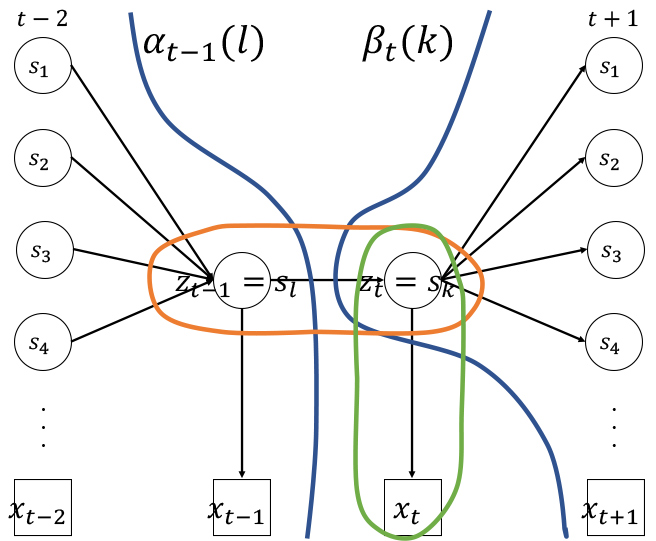
\includegraphics[scale=.38]{HMM_EM.jpg}
\caption{パラメータ$A$を求める計算の概念図}
\label{fig:HMM_A}
\end{center}
\end{figure}
\end{frame}

\begin{frame}{Backward procedure}
\FontMath
$\beta_t(k)$は、動的計画法の一種であるbackward procedureによって、効率的に計算できる
\begin{itemize}
\item[cf.] \href{https://web.stanford.edu/~jurafsky/slp3/A.pdf}{https://web.stanford.edu/\~{}jurafsky/slp3/A.pdf}
\end{itemize}
\begin{align}
\beta_{T-1}(k) & = p(x_T|z_{T-1}=s_k) = \sum_{z_T \in \mathcal{S}} p(z_T|z_{T-1}=s_k)p(x_T|z_T)
= \sum_{l=1}^K A_{s_k, s_l} B_{s_l, x_T}
\\
\beta_{T-2}(k) & = p(x_{T-1},x_T|z_{T-2}=s_k)
= \sum_{z_{T-1} \in \mathcal{S}} p(z_{T-1}|z_{T-2}=s_k)p(x_{T-1}|z_{T-1})p(x_T|z_{T-1})
\notag \\ &
= \sum_{l=1}^K A_{s_k, s_l} B_{s_l,x_{T-1}} \beta_{T-1}(l)
\end{align}
同様に考えて
\begin{align}
\beta_t(k) = \sum_{l=1}^K A_{s_k, s_l} B_{s_l, x_{t+1}} \beta_{t+1}(l)
\end{align}
\end{frame}

\begin{frame}{Forward-backward algorithm}
\begin{itemize}
\item 隠れマルコフモデルについて、$\alpha_t(k)$と$\beta_t(k)$を上述の方法で求めるアルゴリズムを
forward-backwardアルゴリズムと呼ぶ
\begin{itemize}
\item $\alpha_t(k)$がforwardに、$\beta_t(k)$がbackwardに、それぞれ対応
\end{itemize}
\end{itemize}
\end{frame}

\begin{frame}{HMMのEMアルゴリズムのM step (2/3)}
\FontMath
$\sum_{\bm{z}_{1:T}}\mathbbm{1}( z_{t-1} = s_l \wedge z_t = s_k ) 
p(\bm{z}_{1:T} , \bm{x}_{1:T}; A_{\mbox{\scriptsize old}}, B_{\mbox{\scriptsize old}})
= \alpha_{t-1}(l) A_{s_l,s_k} B_{s_k,x_t} \beta_t(k)$より
\begin{align}
A_{s_l, s_k} & \propto \sum_{t=1}^T \alpha_{t-1}(l) A_{s_l,s_k} B_{s_k,x_t} \beta_t(k)
\\
\therefore A_{s_l, s_k} & = 
\frac{ \sum_{t=1}^T \alpha_{t-1}(l) A_{s_l,s_k} B_{s_k,x_t} \beta_t(k) }
{ \sum_{k=1}^K \sum_{t=1}^T \alpha_{t-1}(l) A_{s_l,s_k} B_{s_k,x_t} \beta_t(k) }
\end{align}
次は$B_{s_k,v_w}$を求める。
\begin{align}
\frac{\partial \mathcal{L}(A, B, \lambda, \mu) }{\partial B_{s_k, v_w}}
& = 
\frac{ \sum_{\bm{z}_{1:T}} q(\bm{z}_{1:T}) \sum_{t=1}^T 
\mathbbm{1}( z_t = s_k \wedge x_t = v_w ) }{ B_{z_t,x_t} }
- \mu_k
\end{align}
\begin{align}
\therefore B_{s_k, v_w} = \frac{
\sum_{\bm{z}_{1:T}} q(\bm{z}_{1:T}) \sum_{t=1}^T 
\mathbbm{1}( z_t = s_k \wedge x_t = v_w ) }{
\sum_{w=1}^W \sum_{\bm{z}_{1:T}} q(\bm{z}_{1:T}) \sum_{t=1}^T 
\mathbbm{1}( z_t = s_k \wedge x_t = v_w ) }
\end{align}
\end{frame}

\begin{frame}
\FontMath
\begin{align}
& \sum_{\bm{z}_{1:T}} q(\bm{z}_{1:T}) \sum_{t=1}^T 
\mathbbm{1}( z_t = s_k \wedge x_t = v_w )
= \sum_{t=1}^T \sum_{\bm{z}_{1:T}}   
\mathbbm{1}( z_t = s_k \wedge x_t = v_w ) q(\bm{z}_{1:T})
\notag \\ &
= 
\frac{1}{p(\bm{x}_{1:T}; A_{\mbox{\scriptsize old}}, B_{\mbox{\scriptsize old}})}
\sum_{t=1}^T \sum_{\bm{z}_{1:T}}  
\mathbbm{1}( z_t = s_k \wedge x_t = v_w )
p(\bm{z}_{1:T} , \bm{x}_{1:T}; A_{\mbox{\scriptsize old}}, B_{\mbox{\scriptsize old}})
\end{align}
\begin{align}
\sum_{\bm{z}_{1:T}}  
\mathbbm{1}( z_t = s_k \wedge x_t = v_w )
p(\bm{z}_{1:T} , \bm{x}_{1:T}; A_{\mbox{\scriptsize old}}, B_{\mbox{\scriptsize old}})
= p(z_t = s_k, \bm{x}_{1:T}; A_{\mbox{\scriptsize old}}, B_{\mbox{\scriptsize old}})
\end{align}
\end{frame}


\end{document}